\section{下降—上升方法}
\label{sec:minimax-gda}

内层响应法每轮都要解一个优化问题，代价不小。能不能每轮只算一次两侧的梯度，让$\bm{x}$走一小步下山，同时让$\bm{y}$走一小步上山？本节研究这个最便宜的做法，它在什么情况下行得通，在什么情况下行不通。

\paragraph{主要思想}
设$\bm{X},\bm{Y}$是闭凸集，$f$可微。不再要求内层解到最优，而是让$\bm{y}$只沿内层目标的梯度走一步，$\bm{x}$沿外层方向走一步。这样的方法称为\term{梯度下降—上升}（gradient descent--ascent，GDA）。

两个偏梯度都在旧点计算，称为同时更新：
\begin{equation}
 \begin{aligned}
 \bm{x}^{(t+1)}&=P_{\bm{X}}\bigl(\bm{x}^{(t)}-\alpha\nabla_{\bm{x}}f(\bm{x}^{(t)},\bm{y}^{(t)})\bigr),\\
 \bm{y}^{(t+1)}&=P_{\bm{Y}}\bigl(\bm{y}^{(t)}+\beta\nabla_{\bm{y}}f(\bm{x}^{(t)},\bm{y}^{(t)})\bigr).
 \end{aligned}
 \label{eq:minimax-gda-sim}
\end{equation}

先更新$\bm{x}$，再用新的$\bm{x}$算$\bm{y}$的梯度，称为先后更新：
\begin{equation}
 \begin{aligned}
 \bm{x}^{(t+1)}&=P_{\bm{X}}\bigl(\bm{x}^{(t)}-\alpha\nabla_{\bm{x}}f(\bm{x}^{(t)},\bm{y}^{(t)})\bigr),\\
 \bm{y}^{(t+1)}&=P_{\bm{Y}}\bigl(\bm{y}^{(t)}+\beta\nabla_{\bm{y}}f(\bm{x}^{(t+1)},\bm{y}^{(t)})\bigr).
 \end{aligned}
 \label{eq:minimax-gda-alt}
\end{equation}

两式只有第二行里$\bm{x}$的上标不同，却是不同的递推，下面的例子里轨迹的性质也不同。比较时必须说明用的是哪一种。

\paragraph{计算过程}
用$f(x,y)=xy$，$X=Y=\mathbb{R}$，唯一鞍点是原点。

\needspace{6\baselineskip}
\paragraph{变量}
\begin{itemize}
 \item $x^{(t)},y^{(t)}$：两组变量；
 \item $\alpha,\beta>0$：两侧步长。
\end{itemize}

\paragraph{初始化}
取$(x^{(0)},y^{(0)})$。例中$(x^{(0)},y^{(0)})=(1,0)$，$\alpha=\beta=\frac12$。

\needspace{6\baselineskip}
\paragraph{每轮更新}
\begin{enumerate}
 \item 计算两个偏导数。例中$\partial_xf=y$，$\partial_yf=x$。
 \item 按式~\eqref{eq:minimax-gda-sim}或式~\eqref{eq:minimax-gda-alt}更新。例中同时更新的第一轮
 \[
  x^{(1)}=1-\frac12\cdot0=1,\qquad y^{(1)}=0+\frac12\cdot1=\frac12.
 \]
 第二轮、第三轮分别得到
 \[
  (x^{(2)},y^{(2)})=(0.75,1),\qquad(x^{(3)},y^{(3)})=(0.25,1.375).
 \]
 \item 先后更新的第一轮结果相同，因为$y^{(0)}=0$时$x$不动。第二轮和第三轮分别是
 \[
  (x^{(2)},y^{(2)})=(0.75,0.875),\qquad(x^{(3)},y^{(3)})=(0.3125,1.03125).
 \]
\end{enumerate}

通常的结束条件是步数达到上限，或残差小于容差。例中距离鞍点的平方，同时更新依次为$1,1.25,1.5625,1.953$，每轮乘以$1.25$；先后更新依次为$1,1.25,1.3281,1.161$，有界地上下波动。最终两种更新都没有接近鞍点。下一小节解释原因。

\subsection{旋转现象}
\label{sec:minimax-rotation}

把同时更新用矩阵写出来，记$\bm{z}=(x,y)^\top$，式~\eqref{eq:minimax-gda-sim}成为
\begin{equation}
 \bm{z}^{(t+1)}=\begin{pmatrix}1&-\alpha\\\alpha&1\end{pmatrix}\bm{z}^{(t)}.
 \label{eq:minimax-gda-matrix}
\end{equation}

这个矩阵是一个旋转矩阵乘以$\sqrt{1+\alpha^2}$。两列互相正交，长度都是$\sqrt{1+\alpha^2}$，所以
\begin{equation}
 \lVert\bm{z}^{(t+1)}\rVert_2^2=(1+\alpha^2)\lVert\bm{z}^{(t)}\rVert_2^2.
 \label{eq:minimax-gda-growth}
\end{equation}

对任何固定的$\alpha>0$，距离都按几何级数增长。$\alpha=\frac12$时每轮乘以$1.25$，与上面的数字一致。步长取得再小，也只是增长得慢，不会变成收缩。

几何上，迭代方向是$(-y,x)$，它和位置向量$(x,y)$处处垂直，也就是沿着以原点为圆心的圆的切线方向。沿切线走一小段，总是落到更大的圆上。这像绕着一个圆运动的人每走一步都沿当前切线走直线，路线不是回到原圆，而是向外盘旋。连续时间的方程$\dot{\bm{z}}=(-y,x)$恰好沿圆运动，半径不变；离散化把这个“恰好不靠近”的运动变成了发散。

先后更新的矩阵是
\[
 \begin{pmatrix}1&-\alpha\\\alpha&1-\alpha^2\end{pmatrix},
\]
行列式是$1$，迹是$2-\alpha^2$。$0<\alpha<2$时迹的绝对值小于$2$，两个特征值是模为$1$的共轭复数，迭代既不发散也不收敛。

这一点可以用一个守恒量看得更清楚。令$Q=x^2+y^2-\alpha xy$，记$x^{+}=x-\alpha y$，$y^{+}=y+\alpha x^{+}$。先处理含$y^{+}$的两项：
\[
 (y^{+})^2-\alpha x^{+}y^{+}=y^{+}(y^{+}-\alpha x^{+})=y^{+}y=y^2+\alpha x^{+}y.
\]
再处理剩下的项：
\[
 (x^{+})^2+\alpha x^{+}y=x^{+}(x^{+}+\alpha y)=x^{+}x=x^2-\alpha xy.
\]
两式相加，得到
\[
 (x^{+})^2+(y^{+})^2-\alpha x^{+}y^{+}=x^2+y^2-\alpha xy,
\]
所以$Q$沿迭代不变。$0<\alpha<2$时$Q$是正定二次型，迭代点永远留在同一个椭圆上，既跑不掉也到不了中心。图~\ref{fig:minimax-gda-rotation}(a)(b)画出了两种轨迹。

\begin{BookInlineFigure}
 \centering
 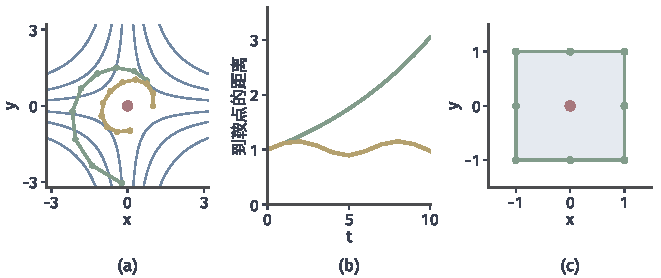
\includegraphics[width=112mm]{figures/05-optimization/07-multiple-criteria-and-nested-optimization/matplotlib/minimax-gda-rotation/figure.pdf}
 \caption{$f=xy$上的下降—上升，蓝线是等高线，红点是鞍点。(a)$\alpha=\frac12$，起点$(1,0)$，$10$步：绿色是同时更新，向外盘旋；黄色是先后更新，留在椭圆上。(b)两种更新到鞍点的距离。(c)盒子$[-1,1]^2$上的投影同时更新，$\alpha=1$，从$(1,0)$出发，$8$步回到起点。}
 \label{fig:minimax-gda-rotation}
\end{BookInlineFigure}

\paragraph{加上约束也不收敛}
把迭代限制在盒子里能防止发散，却不能让它停在鞍点。取$X=Y=[-1,1]$，$\alpha=\beta=1$，从$(1,0)$出发做投影同时更新，投影就是逐分量截断到$[-1,1]$。第一步$x=1-0=1$，$y=0+1=1$；第二步$x=1-1=0$，$y=1+1=2$，截断成$1$。继续算下去，得到
\[
 \begin{aligned}
 (1,0)&\to(1,1)\to(0,1)\to(-1,1)\to(-1,0)\\
 &\to(-1,-1)\to(0,-1)\to(1,-1)\to(1,0).
 \end{aligned}
\]

八步之后回到起点，见图~\ref{fig:minimax-gda-rotation}(c)。由式~\eqref{eq:minimax-box-gap}，循环上的间隙$\lvert x\rvert+\lvert y\rvert$取$1$或$2$，永远不小于$1$。定理~\ref{thm:minimax-theorem}的条件全部满足，鞍点存在，算法却找不到它。存在性定理回答解在不在，不回答某个算法能否到达。

\paragraph{只看一侧的数不足以判断}
图~\ref{fig:minimax-gda-monitor}(a)是同时更新过程中$f(x^{(t)},y^{(t)})$的值。从$t=2$到$t=5$，它从$0.75$一路降到$-1.52$。如果只看这条线，会以为外层目标在稳步下降，而图~\ref{fig:minimax-gda-monitor}(b)显示点正在远离解。$f$的值本来就该由一侧压低、另一侧抬高，它的升降不说明任何问题。

\begin{BookInlineFigure}
 \centering
 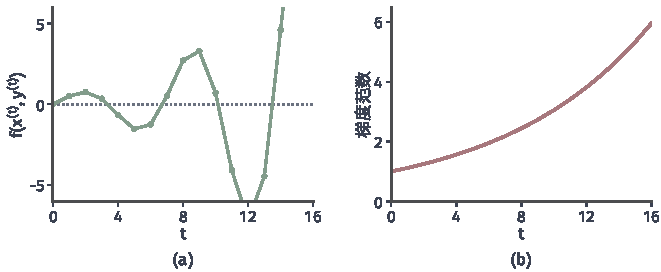
\includegraphics[width=112mm]{figures/05-optimization/07-multiple-criteria-and-nested-optimization/matplotlib/minimax-gda-monitor/figure.pdf}
 \caption{$f=xy$上同时更新的监控量，$\alpha=\frac12$，起点$(1,0)$。(a)绿线是代价$f$的值，在部分时段连续下降，又在更大的幅度上振荡。(b)红线是两侧梯度的范数$\lVert(y,-x)\rVert_2$，它等于到鞍点的距离，持续增长。}
 \label{fig:minimax-gda-monitor}
\end{BookInlineFigure}

反过来，梯度为零也说明不了稳定。对$f=xy$，原点两侧梯度都为零，而且原点就是解，迭代却从任何非零点开始都远离它，一旦有扰动也回不去。对$f=y^2-x^2$，原点两侧梯度也为零，但迭代$x^{+}=(1+2\alpha)x$，$y^{+}=(1+2\alpha)y$从原点附近往外推，原点又不是解。所以驻定只回答“这个点本身怎样”，不回答“迭代会不会留在它附近”，后者要看迭代映射的线性化。

\subsection{响应速度}
\label{sec:minimax-speed}

$f=xy$没有内层曲率，$\bm{y}$没有自己想去的位置。内层有强凹性时，$\bm{y}$就有一个目标$\bm{y}^\star(\bm{x})$，问题变成：$\bm{y}$能否跟上这个随$\bm{x}$移动的目标？

继续用$f=-\frac12x^2+2xy-\frac12y^2$，最优响应是$y=2x$，原点是顺序问题的解。令$\beta=r\alpha$，$r$是两侧步长之比。迭代$\bm{z}^{+}=(\bm{I}-\alpha\bm{J}_r)\bm{z}$的矩阵是
\begin{equation}
 \bm{J}_r=\begin{pmatrix}-1&2\\-2r&r\end{pmatrix}.
 \label{eq:minimax-timescale-matrix}
\end{equation}

$\bm{J}_r$的迹是$r-1$，行列式是$3r$。当$1<r<13$时，判别式$(r-1)^2-12r<0$，两个特征值是共轭复数$\lambda$，满足$\operatorname{Re}\lambda=\frac{r-1}{2}$，$\lvert\lambda\rvert^2=3r$。迭代的模平方是
\[
 \lvert1-\alpha\lambda\rvert^2=1-\alpha(r-1)+3r\alpha^2.
\]

这个量小于$1$，当且仅当
\begin{equation}
 0<\alpha<\frac{r-1}{3r}.
 \label{eq:minimax-timescale-stable}
\end{equation}

$r=1$时模平方是$1+3\alpha^2>1$，任何步长都发散。$r<1$时两个特征值的实部为负，$\lvert1-\alpha\lambda\rvert>1$，同样发散。$r=4$时条件是$\alpha<\frac14$，例如$\alpha=0.1$时模平方是$0.82$。两种选择用同样的$\alpha$，差别只在$y$走得快不快，见图~\ref{fig:minimax-timescale}。

\begin{BookInlineFigure}
 \centering
 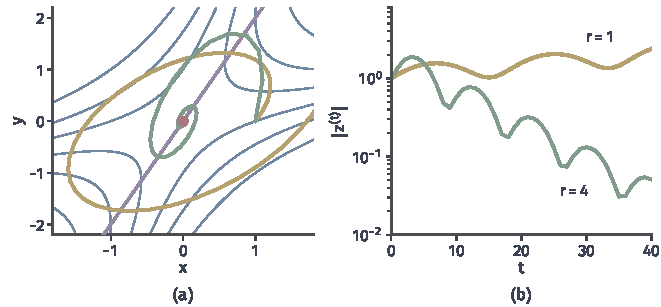
\includegraphics[width=112mm]{figures/05-optimization/07-multiple-criteria-and-nested-optimization/matplotlib/minimax-timescale/figure.pdf}
 \caption{$f=-\frac12x^2+2xy-\frac12y^2$上的同时更新，$\alpha=0.1$，起点$(1,0)$，$40$步。蓝线是等高线，紫线是最优响应$y=2x$，红点是解。黄线$r=1$，两侧同速，$y$跟不上$x$，轨迹向外盘旋。绿线$r=4$，$y$走得快，轨迹贴着紫线向解收敛。(b)到解的距离。}
 \label{fig:minimax-timescale}
\end{BookInlineFigure}

$r$的门槛来自$f$的结构。$\partial_x^2f=-1$是外层变量的负曲率，$\partial_y^2f=-1$是内层变量提供的强凹性。外层独自运动时是往外推的，只有$y$足够快地跟上$y=2x$，外层才看得到$\phi''=3>0$的正曲率。$y$落后时，外层感受到的是$f$在旧$y$上的负曲率，于是被推开。

\paragraph{跟踪误差的递推}
一般情形可以用跟踪误差来刻画这种竞赛。沿用第~\ref{sec:minimax-approx-response}节的条件，记跟踪误差为
\begin{equation}
 e_t=\lVert\bm{y}^{(t)}-\bm{y}^\star(\bm{x}^{(t)})\rVert_2.
 \label{eq:minimax-tracking-error}
\end{equation}

第~\ref{chap:feasible-iterations}章证明过：$\mu$强凸、$L$-光滑的函数上，步长为$1/L$的投影梯度法把到解的距离至少缩小到$\rho=\sqrt{1-\mu/L}$倍。把它用到凸函数$-f(\bm{x},\cdot)$上。

\begin{lemma}[跟踪误差的递推]
\label{lem:minimax-tracking}
设$\bm{x}^{(t+1)}$已经算出，从$\bm{y}^{(t)}$出发在$f(\bm{x}^{(t+1)},\cdot)$上做$K$步步长$1/L$的投影梯度上升，得到$\bm{y}^{(t+1)}$。则
\begin{equation}
 e_{t+1}\leq\rho^{K}\bigl(e_t+\kappa\lVert\bm{x}^{(t+1)}-\bm{x}^{(t)}\rVert_2\bigr).
 \label{eq:minimax-tracking}
\end{equation}
\end{lemma}

\begin{proof}
$K$步投影梯度上升的收缩给出
\[
 e_{t+1}\leq\rho^K\lVert\bm{y}^{(t)}-\bm{y}^\star(\bm{x}^{(t+1)})\rVert_2.
\]
用三角不等式，并由引理~\ref{lem:minimax-response-lipschitz}的$\kappa$-Lipschitz性，
\[
 \lVert\bm{y}^{(t)}-\bm{y}^\star(\bm{x}^{(t+1)})\rVert_2\leq e_t+\kappa\lVert\bm{x}^{(t+1)}-\bm{x}^{(t)}\rVert_2.
\]
两式合起来即得。
\end{proof}

式~\eqref{eq:minimax-tracking}里，$\rho^K$是内层追赶的速度，$\kappa\lVert\bm{x}^{(t+1)}-\bm{x}^{(t)}\rVert_2$是目标跑开的距离。要跟得上，有两种办法：增加$K$，或者减小外层步长。

取$K=1$，看外层步长要小到什么程度。设每步外层移动量是$\alpha\lVert\bm{g}\rVert_2$，$\rho\approx1-\frac{1}{2\kappa}$。递推的稳态是
\[
 e_\infty\approx\frac{\kappa\alpha\lVert\bm{g}\rVert_2}{1-\rho}\approx2\kappa^2\alpha\lVert\bm{g}\rVert_2.
\]

外层梯度的误差约为$Le_\infty$。要让它不超过$\frac12\lVert\bm{g}\rVert_2$，需要$\alpha\lesssim\frac{1}{4\kappa^2L}$，也就是$\alpha/\beta$是$1/\kappa^2$量级。这个推算只是说明量级，不是证明。完整的结论要把式~\eqref{eq:minimax-tracking}和定理~\ref{thm:minimax-inexact-descent}放进同一个势函数，得到的是非凸—强凹问题上求$\phi$的$\epsilon$驻定点需要$O(\kappa^2/\epsilon^2)$量级的梯度读取。该证明篇幅较长，读者可查阅双时间尺度下降—上升的专门分析。

理论的步长是保守的。上例$L=3$，$\kappa=3$，上述量级给出的$\alpha$约为$\frac{1}{108}$，而取$\beta=\frac13$时由式~\eqref{eq:minimax-timescale-stable}可算出实际的稳定范围到$\alpha<\frac16$。保证覆盖的是一个函数类中最差的情形，这与第~\ref{chap:first-order-methods}章步长的保守取法一样。

\paragraph{非凸—非凹情形}
以上依赖强凹性带来的$\kappa$-Lipschitz响应。式~\eqref{eq:minimax-nonconcave}中最优响应在$x=0$处从$-\sqrt2$跳到$\sqrt2$，没有任何Lipschitz常数，内层再快也不能平稳地跟踪。此时必须分别说明三件事：用的是什么步长组合，内层响应求到了什么程度，所报告的驻定概念是什么，第~\ref{sec:minimax-evaluation}节回到这些问题。一般非凸—非凹问题上，下降—上升可能循环，也可能发散，没有与上面同类的保证。
